\documentclass{article}

\usepackage{graphicx}
\usepackage[letterpaper]{geometry}

\graphicspath{{./img/}}

\title{2411 Project 4}
\author{Duncan Wilkie}
\date{15 October 2021}

\begin{document}

\maketitle

\section{Analytical Solution}
The analytical solution to the provided ODE is $V_{exact}(r)=-\frac{W_0}{1+e^{(r-R)/a}}$.
\section{Numerical Method}
We use RK2, implemented in C++, to approximate the solution to the ODE.
\section{Program Analysis}
The program written for this section appears in the script files section. A plot of the results for both step sizes appears below:
\[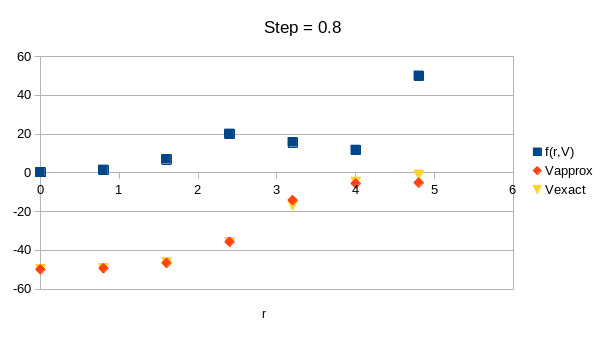
\includegraphics[scale=0.5]{plot1.png}\]
\[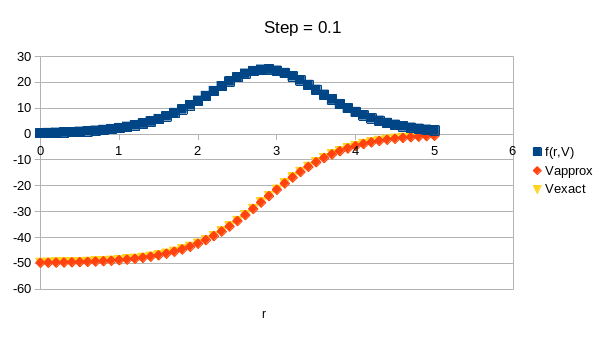
\includegraphics[scale=0.5]{plot2.png}\]
The result shows close tracking of the analytical solution by the numerical, with increased accuracy with smaller step size. Smaller step size greatly affects the value of the approximate derivative, with it blowing up at the end of the 0.8 step size case only.
A semilog plot of the absolute error appears below:
\[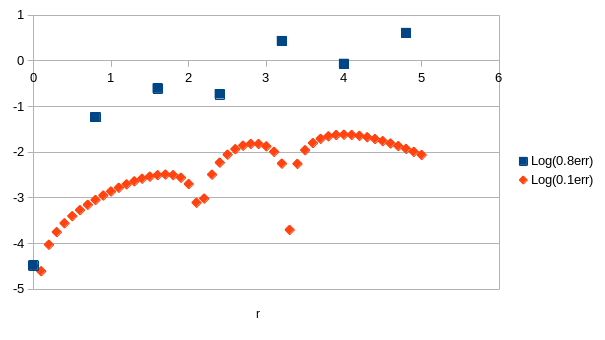
\includegraphics[scale=0.5]{plot3.png}\]
This shows the absolute error is consistently much lower for the smaller step size. For the smaller step size, the log of the absolute error appears to vary with $r$ roughly as $\log(x)$, but with apparent discontinuities at certain points. The absolute error then is roughly $\epsilon = kr\epsilon(r)$, where $\epsilon(r)$ is close to 1 for most $r$ but goes to zero at the points where the discontinuities lie in the semilog plot above.
A plot of the RK4 solution against the exact value with a step of 0.8 appears below.
\[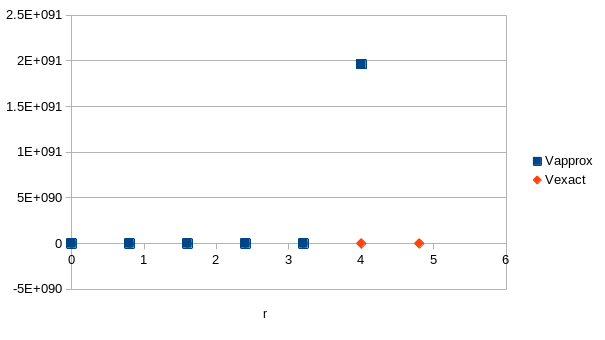
\includegraphics[scale=0.5]{plot4.png}\]
The approximate solution blows up wildly, since the approximation for $f(r, V)$ does as well.
\section{Script Files}
\subsection*{Program 1}
\begin{verbatim}
Script started, file is dwilk14_proj4p1.txt
[dwilk14@tigers ~/Project4]$ cat dwilk14_proj4p1.cpp
#include <cmath>
#include <iostream>
#include <fstream>
#include <utility>
#include <vector>

using namespace std;


double rk2step(double (*f)(double, double), double y0, double t0, double h) {
  double k1 = h * f(t0, y0);
  return h * f(t0 + h / 2, y0 + k1 / 2);
}

double f(double r, double V) {
  double W0 = 50, R = 2.86179, a = 0.5;
  return 1 / (a * W0) * exp((r - R) / a) * pow(V, 2);
}

double Vexact(double r) {
  double W0 = 50, R = 2.86179, a = 0.5;
  return -W0 / (1 + exp((r-R) / a));
}

int main() {
  ofstream outfile;
  outfile.open("output.txt");
  double V = -49.8371, r = 0, b = 5, h = 0.8;

  outfile << "r f(r, V) Vapprox Vexact Verr" << endl;

  outfile << "Step = 0.8" << endl;
  
  while (r <= b) {
    outfile << r << " " << f(r, V) << " " << V  << " " << Vexact(r) << " " \
            << abs(Vexact(r) - V) << endl;
    V += rk2step(f, V, r, h);
    r += h;

  } 

  outfile << "Step = 0.1" << endl;
  
  r = 0;
  h = 0.1;
  V = -49.8371;
  while (r <= b) {
    outfile << r << " " << f(r, V) << " " << V  << " " << Vexact(r) << " " \
            << abs(Vexact(r) - V) << endl;
    V  += rk2step(f, V, r, h);
    r += h;
  }  

  return 0;

}
[dwilk14@tigers ~/Project4]$ g++ dwilk14_proj4p1.cpp -o dwilk14_proj4p1                                                                                                                      
[dwilk14@tigers ~/Project4]$ ./dwilk14_proj4p1
[dwilk14@tigers ~/Project4]$ cp dwilk14_proj4p1.txt /home3/kristina/phys2411/.
[dwilk14@tigers ~/Project4]$ exit
exit
Script done, file is dwilk14_proj4p1.txt
\end{verbatim}

\subsection*{Program 2}
\begin{verbatim}
Script started, file is dwilk14_proj4p2.txt
[dwilk14@tigers ~/Project4]$ cat dwilk14_proj4p2.cpp
#include <cmath>
#include <iostream>
#include <fstream>
#include <utility>
#include <vector>

using namespace std;


double rk4step(double (*f)(double, double), double y0, double t0, double h) {
  double k1 = h * f(t0, y0);
  double k2 = h * f(t0 + h / 2, y0 + k1 / 2);
  double k3 = h * f(t0 + h / 2, y0 + k2 / 2);
  double k4 = h * f(t0 + h, y0 + k3);
  return y0 + k1 / 6 + k2 / 6 + k3 / 6 + k4 / 6;
}

double f(double r, double V) {
  double W0 = 50, R = 2.86179, a = 0.5;
  return 1 / (a * W0) * exp((r - R) / a) * pow(V, 2);
}

double Vexact(double r) {
  double W0 = 50, R = 2.86179, a = 0.5;
  return -W0 / (1 + exp((r-R) / a));
}

int main() {
  ofstream outfile;
  outfile.open("output2.txt");
  double V = -49.8371, r = 0, b = 5, h = 0.8;

  outfile << "r f(r, V) Vapprox Vexact Verr" << endl;

  outfile << "Step = 0.8" << endl;
  
  while (r <= b) {
    outfile << r << " " << f(r, V) << " " << V  << " " << Vexact(r) << " " \
            << abs(Vexact(r) - V) << endl;
    V += rk4step(f, V, r, h);
    r += h;

  } 

  return 0;

}
[dwilk14@tigers ~/Project4]$ g++ dwilk14_proj4p2.cpp -o dwilk14_proj4p2
[dwilk14@tigers ~/Project4]$ ./dwilk14_proj4p2
[dwilk14@tigers ~/Project4]$ cp dwilk14_proj4p2.txt /home3/kristina/phys2411/.
[dwilk14@tigers ~/Project4]$ exit
exit
Script done, file is dwilk14_proj4p2.txt
\end{verbatim}
 \end{document}
%%% Local Variables:
%%% mode: latex
%%% TeX-master: t
%%% End:
